\section{Elastisk net}
I dette afsnit introduceres en shrinkage metode kaldet elastisk net, som kombinerer ridge regression og lasso.
Metoden blev først præsenteret i \citep{zou_hastie}.

Selvom lasso har vist succes i mange tilfælde, har den også nogle begrænsninger:
%
\begin{enumerate}[label=\textnormal{(\arabic*)}]
    \item Hvis $p>n$, da udvælger lasso højst $n$ variable, hvilket kommer af, at lasso er et konvekst optimeringsproblem (KAN DET BEVISES). Derudover er lasso ikke veldefineret medmindre \(\Vert \beta \Vert_1 \leq t\). \label{itm:1}
    \item Hvis der eksisterer en gruppe af variable, som har høj parvis korrelation, da har lasso en tendens til blot at udvælge  én variabel fra denne gruppe og denne variabel udvælges tilfældigt (MÅSKE EKS PÅ DET). \label{itm:2}
    \item Hvis $n>p$ og der er høj korrelation mellem variablerne, da er det empirisk bevist at prædiktions performance af lasso er domineret af ridge regression \citep{lasso}.  \label{itm:3}
\end{enumerate}
%
Målet er at finde en metode, som overkommer ovenstående begrænsninger.
Ridge regression kan håndtere multikollinaritet, da den averages effekten af mutually korrelerede variable.
Men somsagt giver ridge regression ikke en sparse løsning.

Antag responsvariablen er centreret og prædiktorerne er standardiseret, da er det naive elastiske net givet ved
\begin{align}
\hat{\beta}^\text{naivEN} = \argmin_{\beta} \cbr{ \frac{1}{2n} \Vert \y - \X \beta \Vert_2^2 + \lambda_2 \Vert \beta \Vert_2^2 + \lambda_1 \Vert \beta \Vert_1}, \label{eq:EN1}
\end{align}
for \(\lambda_1, \lambda_2 \geq 0\).
Lad \(\alpha = \frac{\lambda_2}{\lambda_1 + \lambda_2}\), da svarer \eqref{eq:EN1} til optimeringsproblemet
\begin{align*}
\hat{\beta}^\text{naivEN} = \argmin_{\beta} \cbr{\frac{1}{2n} \Vert \y - \X \beta \Vert_2^2}, \ \text{underlagt at } \del{1-\alpha} \Vert \beta \Vert_1 + \alpha \Vert \beta \Vert_2^2 \leq t,
\end{align*}
som kan omskrives til et Lagrange problem
\begin{align}
\hat{\beta}^\text{naivEN} =\argmin_{\beta} \cbr{\frac{1}{2n} \Vert \y - \X \beta \Vert_2^2 + \lambda \sbr{(1- \alpha) \Vert \beta \Vert_1 + \alpha \Vert \beta \Vert_2^2}}. \label{eq:4.2}
\end{align}
Hvis $\alpha=0$, da reduceres strafleddet til $\ell_1$-normen svarende til strafleddet for lasso, og hvis $\alpha=1$ reduceres det til den kvadrerede $\ell_2$-norm svarende til strafleddet for ridge regression.
Optimeringsproblemet  \eqref{eq:4.2} er streng konveks for \(\alpha \in [0,1)\), hvilket betyder, at der eksisterer en entydig løsning uafhængigt af korrelationsstrukturen af $\X$.
For  \(\alpha=0\) er problemet konveks, men ikke streng konveks.
Dette ses tydeligt på figur \ref{fig:elastisk}.
%
\begin{figure}[H]
\centering
\scalebox{0.8}{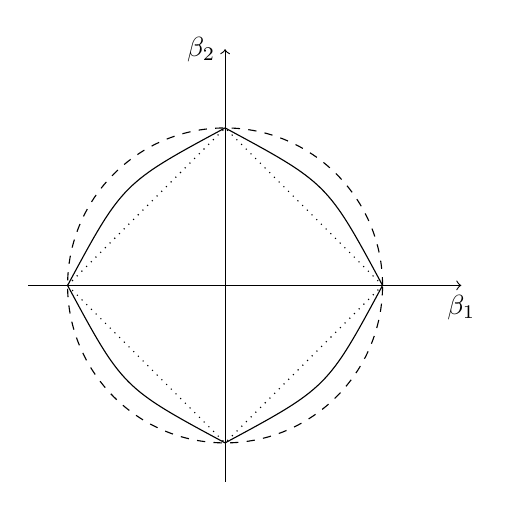
\begin{tikzpicture}
\draw[dashed] (0,0) circle (2cm);
\draw[dotted] (-2,0) -- (0,-2) -- (2,0) -- (0,2) -- (-2,0); 
\draw (-2,0) .. controls (-1.3,1.3) .. (0,2);
\draw (0,2) .. controls (1.3,1.3) .. (2,0);
\draw (-2,0) .. controls (-1.3,-1.3) .. (0,-2);
\draw (0,-2) .. controls (1.3,-1.3) .. (2,0);
\draw [<-] (0,3) node [left] {$\beta_2$}-- (0,-2.5);
\draw[<-] (3,0) node [below] {$\beta_1$} -- (-2.5,0);
\end{tikzpicture}}
\caption[optional short text]{To dimensional illustration af betingelsesområderne for shrinkage metoderne: ridge regression (\tikz[baseline]{\draw[dashed] (0,.5ex)--++(.5,0) ;}), lasso (\tikz[baseline]{\draw[dotted] (0,.5ex)--++(.5,0) ;}) og elastisk net med \(\alpha = 0.5\) (\tikz[baseline]{\draw (0,.5ex)--++(.5,0) ;}). Vi observerer, at singulariteter i hjørnerne og kanterne er streng konveks. Styrken af konveksitet varierer med \(\alpha\).} \label{fig:elastisk}
\end{figure}
%
\begin{figure}[H]
\centering
\begin{minipage}{0.4\linewidth}
\scalebox{0.32}{\includegraphics{fig/crime_lasso.png}}
\end{minipage}
\hspace{0.2cm}
\begin{minipage}{0.4\linewidth}
\scalebox{0.32}{\includegraphics{fig/crime_EN.png}}
\end{minipage}
\caption{Koefficientstierne for henholdsvis lasso (ventre) og elastisk net med \(\alpha=0.3\) (højre) plottet imod \(\ell_1\)-normen for crime data.} \label{fig:crime_koef_EN}
\end{figure}
%
En tre dimensionel illustration af betingelsesområderne for det elastiske net og standard lasso er givet på figur \ref{fig:elastisk_net}.
Heraf ses at det elastiske net har egenskaberne af både $\ell_1$ kuglen og $\ell_2$ kuglen: de skarpe hjørner og kanter opfordrer til variable udvælgelse, mens de kurvede konturer opfordrer stærk korreleret variable til at dele koefficienter.
%
\begin{figure}[H]
\centering
 \scalebox{0.5}{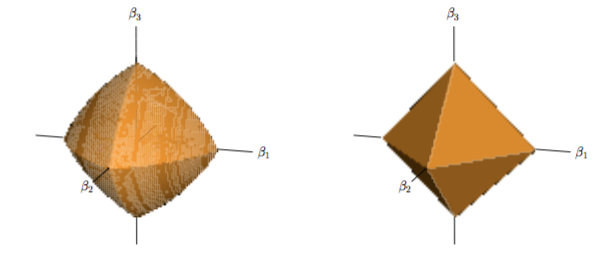
\includegraphics{fig/elastisk_net.jpg}}
\caption{Kuglen for elastisk net med \(\alpha=0.7\) (venstre) og \(\ell_1\) kuglen (højre) i tre dimensioner.}
\label{fig:elastisk_net}
\end{figure}
%
Det viser sig, at optimeringsproblemet for naive elastisk net kan transformeres til et ækvivalent lasso problem på augmented data.
%
\begin{lem} \label{lem:elastisk_net}
Givet data \(\del{\y, \X}\) og parametrene \(\del{\lambda_1, \lambda_2}\), defineres et augmented datasæt 
\begin{align*}
\X^* = \del{1 + \lambda_2}^{-1/2} \begin{bmatrix}
\X \\ \sqrt{\lambda_2} \mathbf{I}
\end{bmatrix}, \quad \y^* = \begin{bmatrix}
\y \\ \mathbf{0}
\end{bmatrix},
\end{align*}
hvor \(\X^* \in \mathbb{R}^{\del{n+p} \times p}\) og \(\y^* \in \mathbb{R}^{n+p}\).
Lad \(\gamma = \frac{\lambda_1}{\sqrt{1+\lambda_2}}\) og \(\beta^* = \sqrt{1+\lambda_2} \beta^\text{naivEN}\), da kan \eqref{eq:EN1} omskrives til
\begin{align*}
\hat{\beta}^* = \argmin_{\beta^*} \cbr{\frac{1}{2n} \Vert \y^* - \X^* \beta^* \Vert_2^2 +\gamma \Vert \beta^* \Vert_1},
\end{align*}
hvor
\begin{align*}
\hat{\beta}^\text{naivEN} = \frac{1}{\sqrt{1+\lambda_2}} \hat{\beta}^*.
\end{align*}
\end{lem}
%
Beviset følger af simpel algebra og er derfor undladt.
Da \(\X^*\) har rang \(p\), kan metoden i princippet altid vælge alle \(p\) prædiktorer.
Dermed er naiv elastisk net ikke begrænset til blot at vælge \(n\) prædiktorer hvis \(p > n\), som er tilfældet for lasso som beskrevet i punkt \ref{itm:1}.
Lemma \ref{lem:elastisk_net} viser også, at naiv  elastisk net udfører variabel udvælgelse svarende til lasso.
%
\begin{lem}
Hvis \(\X\) er ortogonal, da gælder, at
\begin{align}
\hat{\beta}_j^\text{ridge} &= \frac{\hat{\beta}_j^\text{OLS}}{1+\lambda_2}, \label{eq:orto_ridge} \\
\hat{\beta}_j^\text{lasso} &= \text{sign} \del{\hat{\beta}_j^\text{OLS}} \del{\left\vert \hat{\beta}_j^\text{OLS} \right\vert - \lambda_1}_+, \label{eq:orto_lasso} \\
\hat{\beta}_j^\text{naivEN} &= \text{sign} \del{\hat{\beta}_j^\text{OLS}} \frac{\del{\left\vert \hat{\beta}_j^\text{OLS} \right\vert - \lambda_1}_+}{1+\lambda_2}. \label{eq:orto_naivEN}
\end{align}
Figur \ref{fig:elastisk2} viser de operationelle egenskaber af ridge regression, lasso og naiv elastisk net, hvis \(\X\) er ortogonal. Heraf ses det også at naiv elastisk net er en two-stage procedure, først har vi en ridge lignende shrinkage, som efterfølges af en lasso lignende thresholding.
%
\begin{figure}[H]
\centering
\scalebox{0.8}{\begin{tikzpicture}
\draw[loosely dotted] (-3,-3) -- (3,3);
\draw[dotted] (-3,-2) -- (3,2);
\draw (-3,-1.5) -- (-0.75,0) -- (0.75,0) -- (3,1.5);
\draw[dashed] (-3,-2.2) -- (-0.75,0) -- (0.75,0) -- (3,2.2); 
\draw [<-] (0,3.5) node [left] {$\widehat{\beta}$}-- (0,-3.5);
\draw[<-] (3.5,0) node [below] {$\beta$} -- (-3.5,0);
\end{tikzpicture}
}
\caption[optional short text]{Eksakte løsninger for ridge regression (\tikz[baseline]{\draw[dotted] (0,.5ex)--++(.5,0) ;}), lasso (\tikz[baseline]{\draw[dashed] (0,.5ex)--++(.5,0) ;}) og naiv elastisk net (\tikz[baseline]{\draw (0,.5ex)--++(.5,0) ;}), hvis \(\X\) er ortogonal (\tikz[baseline]{\draw[loosely dotted] (0,.5ex)--++(.5,0) ;} OLS) for parametrene \(\lambda_1=2\) og \(\lambda_2=1\).} \label{fig:elastisk2}
\end{figure}
%
\end{lem}
%
\begin{proof}
Ridge estimatoren i det ortogonale tilfælde \eqref{eq:orto_ridge} følger direkte udfra ridge estimatoren \eqref{eq:ridge_estimator}, da \(\X^T \X = \mathbf{I}\) og \(\hat{\beta}^\text{OLS} = \X^T \y\).
For at bevise lasso estimatoren i det ortogonale tilfælde \eqref{eq:orto_lasso}, omskrives lasso problemet \eqref{eq:2.5} til følgende
\begin{align*}
\hat{\beta}^\text{lasso} &= \argmin_{\beta} \cbr{\frac{1}{2n} \del{\y - \X \beta}^T \del{\y - \X \beta} + \lambda_1 \vert \beta \vert} \\
&= \argmin_{\beta} \cbr{\frac{1}{2n} \del{\y^T \y - 2 \beta^T \X^T \y + \beta^T \X^T \X \beta} + \lambda_1 \vert \beta \vert} \\
&= \argmin_{\beta} \cbr{\frac{1}{2n} \del{ - 2 \beta^T \hat{\beta}^\text{OLS} + \beta^T \beta} + \lambda_1 \vert \beta \vert}.
\end{align*}
Lad os blot betragte indeks \(j\) af lasso estimatoren
\begin{align*}
\hat{\beta}_j^\text{lasso} = \argmin_{\beta_j} \cbr{\frac{1}{2n} \del{ - 2 \beta_j \hat{\beta}_j^\text{OLS} + \beta_j^2} + \lambda_1 \vert \beta_j \vert}.
\end{align*}
Vi differentierer
\begin{align*}
\frac{\partial}{\partial \beta_j} \del{\frac{1}{2n} \del{ - 2 \beta_j \hat{\beta}_j^\text{OLS} + \beta_j^2} + \lambda_1 \vert \beta_j \vert}
=-\hat{\beta}^\text{OLS} + \beta_j + \begin{cases}
-\lambda_1 \quad &\beta_j < 0 \\
[-\lambda_1, \lambda_1] & \beta_j = 0 \\
\lambda_1 & \beta_j >0 
\end{cases},
\end{align*}
hvor vi ser bort fra faktoren \(\frac{1}{n}\), da denne er uden betydning under maksimering, sætter udtrykket lig \(0\) og isolerer for \(\hat{\beta}_j\)
\begin{align*}
\hat{\beta}_j^\text{lasso} &= \hat{\beta}_j^\text{OLS} - \begin{cases}
-\lambda_1 \quad &\beta < 0 \\
[-\lambda_1, \lambda_1] & \beta = 0 \\
\lambda_1 & \beta >0 
\end{cases} \\
&= \begin{cases}
\hat{\beta}_j^\text{OLS} - \lambda_1, \quad &\hat{\beta}_j^\text{OLS} > \lambda_1 \\
0, &\hat{\beta}_j^\text{OLS} \leq \lambda_1 \\
\hat{\beta}_j^\text{OLS} + \lambda_1, \quad &\hat{\beta}_j^\text{OLS} < - \lambda_1
\end{cases}. 
\end{align*}
Hvoraf vi får, at \(\hat{\beta}_j^\text{lasso} = S_{\lambda_1} \del{ \hat{\beta}_j^\text{OLS}} \), som fuldfører beviset.
Afslutningsvis følger naiv elastisk net estimatoren i det ortogonale tilfælde \eqref{eq:orto_naivEN} af \eqref{eq:orto_ridge} og \eqref{eq:orto_lasso}, da denne er en kombination heraf.
\end{proof}
%
Hvis vi har en gruppe af højt korreleret variable, da vil lasso blot udvælge én variabel og den udvælges tilfældigt, som nævnt i punkt \ref{itm:2}.
Men naiv elastisk net udvælger alle variable i denne gruppe, som vi nu vil vise. 
En regression metode udviser denne evne, hvis regressions koeffcienterne af en gruppe af højt korreleret variable er approksimativt ens.
%
\begin{lem} \label{lem:elastisk_net2}
Lad os betragte
\begin{align}
\hat{\beta} = \argmin_\beta \Vert \y - \X \beta \Vert_2^2 + \lambda J \del{\beta}, \label{eq:EN10}
\end{align}
hvor \(J \del{\cdot}\) er positiv for \(\beta \neq 0\).
Antag \(\x_i = \x_j\), for \(i, j = 1, \ldots, p\).
\begin{enumerate}[label=\alph*)]
\item Hvis \(J \del{\cdot}\) er streng konveks, da er \(\hat{\beta}_i = \hat{\beta}_j\), for alle \(\lambda \geq 0\).
\item Hvis \(J \del{\beta} = \Vert \beta \Vert_1\), da er \(\hat{\beta}_i \hat{\beta}_j \geq 0\) og \(\hat{\beta}^*\) er optimum af \ref{eq:EN10}, hvor
\begin{align*}
\hat{\beta}_k^* = \begin{cases}
\hat{\beta}_k & k \neq i \text{ og } k \neq j, \\
\del{\hat{\beta}_i + \hat{\beta}_j} s & k = i, \\
\del{\hat{\beta}_i + \hat{\beta}_j} \del{1-s} & k = j,
\end{cases}
\end{align*}
for ethvert \(s \in \sbr{0,1}\).
\end{enumerate}
\end{lem}
%
\begin{proof}
Først bevises a).
Fasthold \(\lambda > 0\).
Hvis \(\hat{\beta}_i \neq \hat{\beta}_j\), lad os betragte \(\hat{\beta}^*\) som
\begin{align*}
\hat{\beta}_k^* = \begin{cases}
\hat{\beta}_k & k \neq i \text{ og } k \neq j, \\
\frac{1}{2} \del{\hat{\beta}_i + \hat{\beta}_j} & k = 1 \text{ eller } k = j.
\end{cases}
\end{align*}
Da \(\x_i = \x_j\), må vi have at \(\X \hat{\beta}^* = \X \hat{\beta}\) og dermed \(\Vert \y - \X \hat{\beta}^* \Vert_2^2 = \Vert \y - \X \hat{\beta} \Vert_2^2\).
Men da \(J \del{\cdot}\) er streng konveks, må vi have, at \(J \del{\hat{\beta}^*} < J \del{\hat{\beta}}\).
Dermed kan \(\hat{\beta}\) være optimum af \eqref{eq:EN10}, som er en modstrid.
Derfor må vi have at \(\hat{\beta}_i = \hat{\beta}_j\).

Herefter bevises b).
Hvis \(\hat{\beta}_i \hat{\beta}_j < 0\), lad os igen betragte \(\hat{\beta}^*\) som ovenfor.
Da ser vi, at \(\vert \hat{\beta}^* \vert < \vert \hat{\beta} \vert\), så \(\hat{\beta}\) kan ikke være en lasso løsning.
MANGLER NOGET!
\end{proof}
Lemma \ref{lem:elastisk_net2} giver altså at streng konveksitet sikrer gruppe effekt hvis vi har identitiske prædiktorer, mens lasso ikke engang har en entydig løsning.
Elastisk net med \(\lambda_2 > 0\) er streng konveks, og har dermed egenskaben i????.


\begin{thm} \label{thm:elastisk_net}
Givet data \(\del{\y, \X}\) og parametrene \(\del{\lambda_1, \lambda_2}\), hvor responsvariablen er centreret og prædiktorerne er standardiseret.
Lad \(\hat{\beta} \del{\lambda_1, \lambda_2}\) være estimatet for naiv elastisk net.
Antag \(\hat{\beta}_i \del{\lambda_1, \lambda_2} \hat{\beta}_j \del{\lambda_1, \lambda_2} > 0\).
Definer
\begin{align*}
D_{\lambda_1, \lambda_2} \del{i,j} = \frac{1}{\Vert \y \Vert_1} \vert \hat{\beta}_i \del{\lambda_1, \lambda_2} - \hat{\beta}_j \del{\lambda_1, \lambda_2} \vert,
\end{align*}
da er
\begin{align}
D_{\lambda_1, \lambda_2} \del{i,j} \leq \frac{1}{\lambda_2} \sqrt{2 \del{1-\rho}}, \label{eq:EN5}
\end{align}
hvor \(\rho = \mathbf{x}_i^T \mathbf{x}_j\) er den empiriske korrelation.
\end{thm}
\begin{proof}
Hvis \(\hat{\beta}_i \del{\lambda_1, \lambda_2} \hat{\beta}_j \del{\lambda_1, \lambda_2} > 0\), da er både \(\hat{\beta}_i \del{\lambda_1, \lambda_2}\) og \(\hat{\beta}_j \del{\lambda_1, \lambda_2}\) ikke-nul og der må gælder, at \(\text{sign} \cbr{\hat{\beta}_i \del{\lambda_1, \lambda_2}} = \text{sign} \cbr{\hat{\beta}_j \del{\lambda_1, \lambda_2}}\).
Lad \(L \del{\lambda_1,\lambda_2, \beta} = \frac{1}{2n} \Vert \y - \X \beta \Vert_2^2 + \lambda_2 \Vert \beta \Vert_2^2 + \lambda_1 \Vert \beta \Vert_1\), således at  \(\arg \min_{\beta} \cbr{L \del{\lambda_1,\lambda_2, \beta}}\) svarer til \eqref{eq:EN1}.
Da må \(\hat{\beta} \del{\lambda_1, \lambda_2}\) opfylde, at
\begin{align*}
\frac{\partial L \del{\lambda_1,\lambda_2, \beta} }{\partial \beta_k} \Bigr|_{\beta = \hat{\beta} \del{\lambda_1, \lambda_2}}=0, \text{ hvis } \hat{\beta}_k \del{\lambda_1, \lambda_2} \neq 0.
\end{align*}
Derfor har vi, at
\begin{align}
-\frac{1}{n} \mathbf{x}_i^T \del{\y - \X \hat{\beta} \del{\lambda_1, \lambda_2}} +  2 \lambda_2 \hat{\beta}_i \del{\lambda_1, \lambda_2} + \lambda_1 \text{sign} \cbr{\hat{\beta}_i \del{\lambda_1, \lambda_2}} &= 0, \label{eq:EN2}\\
-\frac{1}{n} \mathbf{x}_j^T \del{\y - \X \hat{\beta} \del{\lambda_1, \lambda_2}} + 2 \lambda_2 \hat{\beta}_j \del{\lambda_1, \lambda_2} + \lambda_1 \text{sign} \cbr{\hat{\beta}_j \del{\lambda_1, \lambda_2}} &= 0. \label{eq:EN3}
\end{align}
Vi subtraherer \eqref{eq:EN3} fra \eqref{eq:EN2} og finder, at
\begin{align*}
\del{\mathbf{x}_j^T-\mathbf{x}_i^T} \del{\y - \X \hat{\beta} \del{\lambda_1, \lambda_2}} + \lambda_2 \del{\hat{\beta}_i \del{\lambda_1, \lambda_2} - \hat{\beta}_j \del{\lambda_1, \lambda_2}} =0,
\end{align*}
som er ækvivalent med
\begin{align}
\hat{\beta}_i \del{\lambda_1, \lambda_2} - \hat{\beta}_j \del{\lambda_1, \lambda_2} = \frac{1}{\lambda_2} \del{\mathbf{x}_i^T-\mathbf{x}_j^T} \hat{r}\del{\lambda_1, \lambda_2}, \label{eq:EN4}
\end{align}
hvor \(\hat{r}\del{\lambda_1, \lambda_2} = \y - \X  \hat{\beta} \del{\lambda_1, \lambda_2}\) er en vektor af residualer.
Da \(\X\) er standardiseret, har vi, at \(\Vert \mathbf{x}_i - \mathbf{x}_j \Vert_2^2=2 \del{1-\rho}\), hvor \(\rho = \mathbf{x}_i^T \mathbf{x}_j\).
Af \eqref{eq:EN1} må vi have, at
\begin{align*}
L \del{\lambda_1,\lambda_2, \hat{\beta}\del{\lambda_1, \lambda_2}} \leq L \del{\lambda_1,\lambda_2, \beta = 0},  
\end{align*}
dvs
\begin{align*}
\frac{1}{2n} \Vert \hat{r} \del{\lambda_1, \lambda_2} \Vert_2^2 + \lambda_2 \Vert \hat{\beta} \del{\lambda_1, \lambda_2} \Vert_2^2 + \lambda_1 \Vert \hat{\beta} \del{\lambda_1, \lambda_2} \Vert_1 \leq \frac{1}{2n} \Vert \y \Vert_2^2.  
\end{align*}
Dermed er \(\vert \hat{r} \del{\lambda_1, \lambda_2} \vert \leq \vert \y \vert\) og \eqref{eq:EN4} medfører, at
\begin{align*}
D_{\lambda_1, \lambda_2} \del{i,j} \leq \frac{1}{\lambda_2} \frac{\vert \hat{r} \del{\lambda_1, \lambda_2} \vert}{\vert \y \vert} \vert \mathbf{x}_i - \mathbf{x}_j \vert  \leq \frac{1}{\lambda_2} \sqrt{2 \del{1-\rho}}.
\end{align*}
\end{proof}
Mængden \(D_{\lambda_1, \lambda_2} \del{i,j}\) betegner differensen mellem koefficient stierne af prædiktor \(i\) og \(j\).
Hvis \(\mathbf{x}_i\) og \(\mathbf{x}_j\) er højt korreleret, dvs \(\rho \approx 1\), giver sætning \ref{thm:elastisk_net}, at differensen mellem koefficient stierne af prædiktor \(i\) og \(j\) er næsten 0.
Den øvre grænse i \eqref{eq:EN5} giver en kvantitativ beskrivelse af denne gruppering effekt som naiv elastisk net har.

Empiriske resultater har vist, at naiv elastisk net ikke er tilfredsstillende, medmindre den er tæt på enten ridge regression eller lasso.
Derfor kaldes den \textit{naiv}.
Som nævnt tidligere bestemmes en metodes prædiktions performance gennem bias-variance tradeoff. 
Naiv elastisk net er en two-stage procedure. For ethvert fast \(\lambda_2\) finder vi først ridge regression koefficienterne, og derefter shrinkages langs lasso koefficient løsningsstien. Derfor inkluderes en dobbelt shrinkage.
Double shrinkage reducerer ikke variansen meget og introducere unødvendig ekstra bias i forhold til ridge regression eller lasso.
Derfor introduceres blot elastisk net, som korrigerer for denne dobbelt skrinkage.

I lemma \ref{lem:elastisk_net} fandt vi, at naiv elastisk net løser følgende 
\begin{align}
\hat{\beta}^* = \argmin_{\beta^*} \cbr{\frac{1}{2n} \Vert \y^* - \X^* \beta^* \Vert_2^2 + \frac{\lambda_1}{\sqrt{1+\lambda_2}} \Vert \beta^* \Vert_1}. \label{eq:EN8}
\end{align}
Estimaterne for elastisk net (korrigeret) er defineret ved
\begin{align*}
\hat{\beta}^\text{EN} = \sqrt{1+\lambda_2} \hat{\beta}^*.
\end{align*}
Da \(\hat{\beta}^\text{naivEN} = \frac{1}{\sqrt{1+\lambda_2}} \hat{\beta}^*\), har vi, at
\begin{align*}
\hat{\beta}^\text{EN} = \del{1+\lambda_2} \hat{\beta}^\text{naivEN}.
\end{align*}
Dermed er elastisk net koefficienterne faktisk reskaleret naiv elastisk net koefficienter.
Denne transformation bevarer variabel udvælgelsen af naiv elastisk net og er den simpleste måde at annullere det ekstra shrinkage.
Derfor er egenskaberne for naiv elastiske net, som er beskrevet i dette afsnit, stadig gældende for elastisk net.
%
\begin{thm} \label{thm:elastisk_net2}
Givet data \(\del{\y, \X}\) og parametrene \(\del{\lambda_1, \lambda_2}\), da er estimaterne for elastisk net givet ved
\begin{align}
\hat{\beta}^\text{EN} = \argmin_\beta \cbr{ \frac{1}{2n} \del{\beta^T \del{\frac{\X^T \X + \lambda_2 \mathbf{I}}{1 + \lambda_2}} \beta - 2 \y^T \X \beta} + \lambda_1 \Vert \beta \Vert_1}. \label{eq:EN6}
\end{align}
\end{thm}
\begin{proof}
Af ligning \eqref{eq:EN8} har vi, at
\begin{align}
\hat{\beta}^\text{EN} &= \argmin_{\beta} \cbr{\frac{1}{2n} \left\Vert \y^* - \X^* \frac{\beta}{\sqrt{1+\lambda_2}} \right\Vert_2^2 + \frac{\lambda_1}{\sqrt{1+\lambda_2}} \left\Vert \frac{\beta}{\sqrt{1+\lambda_2}} \right\Vert_1} \nonumber \\
&=\argmin_{\beta} \cbr{\frac{1}{2n} \del{\beta^T \del{\frac{\X^{*^T} \X^*}{1+\lambda_2}} \beta - 2 \frac{\y^{*^T} \X^* \beta}{\sqrt{1+\lambda_2}} + \y^{*^T} \y^*} + \frac{\lambda_1 \Vert \beta \Vert_1}{1+\lambda_2}}. \label{eq:EN9}
\end{align}
Følgende identiteter
\begin{align*}
\X^{*^T} \X^* &= \frac{\X^T \X + \lambda_2 \mathbf{I}}{1+ \lambda_2}, \\
\y^{*^T} \X^* &= \frac{\y^T \X}{\sqrt{1+\lambda_2}} ,\\
\y^{*^T} \y^* &= \y^T \y, 
\end{align*}
indsættes i \eqref{eq:EN9}, og vi får, at
\begin{align*}
\hat{\beta}^\text{EN} &= \argmin_{\beta} \cbr{\frac{1}{2n} \del{\beta^T \del{\frac{\X^T \X + \lambda_2 \mathbf{I}}{\del{1+\lambda_2}^2}} \beta - 2 \frac{\y^T \X \beta}{1+\lambda_2} + \y^T \y} + \frac{\lambda_1 \Vert \beta \Vert_1}{1+\lambda_2}} \\ 
%&= \argmin_{\beta} \cbr{\frac{1}{2n} \frac{1}{1+\lambda_2} \del{\beta^T \del{\frac{\X^T \X + \lambda_2 \mathbf{I}}{1+ \lambda_2}} \beta - 2 \y^T \X \beta + \lambda_1 \Vert \beta \Vert_1} + \y^T \y} \\
&= \argmin_{\beta} \cbr{ \frac{1}{2n} \del{\beta^T \del{\frac{\X^T \X + \lambda_2 \mathbf{I}}{1+ \lambda_2}} \beta - 2 \y^T \X \beta} + \lambda_1 \Vert \beta \Vert_1},
\end{align*}
hvor \(\y^T \y= 0 \).
\end{proof}
%
Estimatoren for lasso kan omskrives til
\begin{align}
\hat{\beta}^\text{lasso} = \argmin_\beta \cbr{ \frac{1}{2n} \del{ \beta^T \del{\X^T \X} \beta - 2 \y^T \X \beta } + \lambda_1 \Vert \beta \Vert_1}, \label{eq:EN7}
\end{align}
derfor fortolker sætning \ref{thm:elastisk_net2} elastisk net som en stabil version af lasso.
Lad \(\hat{\Sigma} = \X^T \X\) være den empiriske korrelationsmatrix og
\begin{align*}
\frac{\X^T \X + \lambda_2 \mathbf{I}}{1 + \lambda_2} = (1-\gamma) \hat{\Sigma} + \gamma \mathbf{I},
\end{align*}
hvor \(\gamma=\frac{\lambda_2}{1+\lambda_2}\) shrinks \(\hat{\Sigma}\) mod identitetsmatricen.
Ligning \eqref{eq:EN6} og \eqref{eq:EN7} viser, at reskalere elastisk net er ækvivalent med at erstatte \(\hat{\Sigma}\) med dens shrunken version i lasso.


Somsagt er lasso et specialtilfælde af elastisk net med \(\lambda_2=0\). 
Et andet interessant specialtilfælde er når \(\lambda_2 \rightarrow \infty\).
Af sætning \ref{thm:elastisk_net2} gælder, at \(\hat{\beta}^\text{EN} \rightarrow \hat{\beta} \del{\infty}\) når \(\lambda_2 \rightarrow \infty\), hvor
\begin{align*}
\hat{\beta} \del{\infty} = \argmin_\beta \cbr{\frac{1}{2n} \del{\beta^T \beta - 2 \y^T \X \beta} + \lambda_1 \Vert \beta \Vert_1}.
\end{align*}
\(\hat{\beta} \del{\infty}\) har en simpel lukket løsning, som er givet ved
\begin{align*}
\hat{\beta} \del{\infty}_i = S_{\lambda_1} \del{\y^T \mathbf{x}_i}=\text{sign} \del{\y^T \mathbf{x}_i} \del{\left\vert \y^T \mathbf{x}_i \right\vert - \lambda_1}_+
\end{align*}
for \(i = 1, \ldots, p\).
Vi har, at \(\y^T \mathbf{x}_i\) er en univariat regressions koefficient af den \(i\)'te prædiktor og \(\hat{\beta} \del{\infty}\) er estimaterne som fås udfra soft thresholding på univariater regressions koefficienter.
En univariat soft thresholding ignorerer afhængighedsstrukturen mellem prædiktorerne og behandler dem som uafhængige variable.
%Elastisk net er en natur bro imellem bridges og lasso.

\subsection{Udregning af elastisk net}
Somsagt er optimeringsproblemet for det naive elastiske net \eqref{eq:4.2} konveks og dermed kan flere optimeringsmetoder anvendes til at løse det.

\subsubsection{Coordinat descent}
Opdateringerne for coordinate descent er blot en simpel udvidelse af dem for standard lasso i sektion \ref{subsec:udregning_lasso}.

For standardiseret prædiktorer og en centeret responsvariabel er coordinate descent opdateringen for $j$'te koefficient er givet ved
\begin{align}
\hat{\beta}_j = \frac{S_{\lambda \alpha} \del{\beta_j^*}}{1 + \lambda (1-\alpha)}, \label{eq:4.4}
\end{align}
hvor $S_\mu(z)=\text{sign}(z)(z-\mu)_+$ er soft-thresholding operatoren, \(\beta_j^* = \frac{1}{n} \sum_{i=1}^n x_{ij} r_{ij}\) og $r_{ij}=y_i - \sum_{k \neq j} x_{ik} \hat{\beta}_k$ er den partial residual. 
Vi gennemløber opdateringen \eqref{eq:4.4} indtil konvergens.

%Igen centreres prediktorerne \(x_{ij}\), hvoraf den optimale skæring er givet ved \(\hat{\beta}_0=\bar{y}=\frac{1}{n} \sum_{j=1}^n y_j\).
%Efter at have løst \(\hat{\beta}_0\), udregnes den optimale vektor \(\hat{\beta}= \del{\hat{\beta}_1, \ldots, \hat{\beta}_p}\).
%
%Coordinate descent opdateringen for $j$'te koefficient er givet ved
%\begin{align}
%\hat{\beta}_j = \frac{S_{\lambda \alpha} \del{\sum_{i=1}^n r_{ij} x_{ij}}}{\sum_{i=1}^n x_{ij}^2 + \lambda (1-\alpha)}, \label{eq:4.4}
%\end{align} 
%hvor $S_\mu(z)=\text{sign}(z)(z-\mu)_+$ er soft-thresholding operatoren og $r_{ij}=y_i - \hat{\beta}_0 - \sum_{k \neq j} x_{ik} \hat{\beta}_k$ er den partial residual.
%Vi gennemløber opdateringen \eqref{eq:4.4} indtil konvergens.


\subsubsection{LARS}
Algoritmen LARS-EN kan anvendes til at løse elastisk net, som er baseret på algoritmen LARS, der præsenteres i \cite{efron}.
Af lemma \ref{lem:elastisk_net} ved vi, at for ethvert fast \(\lambda_2\) er elastisk net problemet ækvivalent med lasso problemet på augmented data.
Derfor kan LARS algoritmen anvendes direkte til at finde en elastisk net løsningssti med computermæssig omkostninger som et OLS fit.
Bemærk at for \(p \gg n\), har augmented data \(p+n\) observationer og \(p\) variable, hvilket kan forsinket udregningerne.

Vi kan yderligere lette udregningerne ved at drage fordel af sparsititeten af \(\X^*\) som er afgørende for \(p \gg n\)

Hvis algoritmen stoppes efter \(m\) steps, da kræves \(O \del{m^3 + pm^2}\) operationer.

Løsningsstien for elastisk net er piecewise linear.

For elastisk net har vi to tuning parametre. 
Typisk vælges en lav værdi for \(\lambda_2\), f.eks. \(\del{0,0.01,0.1,1,10,100}\).
For hvert \(\lambda_2\), giver LARS-EN hele løsningsstien for elastisk net.
Den anden tuning parameter \(\lambda_1\) vælges af en 10 fold krydsvalidering.
Den valgte \(\lambda_2\) er den som giver den mindste krydsvalideringsfejl.

For hvert \(\lambda_2\), svarer de computermæssige omkostninger af en 10 fold krydsvalidering til 10 OLS fits.
Derfor er en to-dimensional krydsvalidering computermæssigt sparsommelig for \(n > p\).
Hvis \(p \gg n\), vokser omkostningerne lineært med \(p\).

\subsection{Entydighed og konsistens af elastisk net}
Opfylder den orakel egenskaberne?
\newpage
